%\documentclass[11pt]{article}
%\input{header_old.tex}
%\usepackage[none]{hyphenat} 
%\usepackage{tikz}
%\usepackage{pgfplots}
%\usepackage[normalem]{ulem}
%\usepackage[hidelinks]{hyperref}

% Instructions to change to html version:
% Comment out:
%  minipage, multicols,columnbreak, mathbf, hrule
% Replace all: \begin{minipage}% \end{minipage} %\begin{multicols}  %\end{multicols}  %%\columnbreak %% \begin{framed} %\end{framed} %%\hrule
% Replace \mathbf with \boldsymbol
% Replace $$ with \[ or \]and $ with \( or \)
% Enclose graphics in figure environments and add captions
% 			search \includegraphics
% Re-tag \df environments as sections, subsections, etc.
% Command Line Code to Create html version:
%First: pdflatex -shell-escape filename.tex                                   
%Second, for each figure: inkscape "filename-figure1.pdf" -o "filename-figure1.png"
% Third: htlatex filename.tex "ht5mjlatex.cfg, charset=utf-8" " -cunihtf -utf8"

\documentclass[10pt]{article}

%\usepackage{tikz, pgf,pgfplots,wasysym,array}
%\usepackage{wasysym,array}

\usepackage{amsmath,amssymb}
\usepackage[hidelinks]{hyperref}

\ifdefined\HCode
  \def\pgfsysdriver{pgfsys-tex4ht-updated.def}
\fi 
%\ifdefined\HCode
%  \def\pgfsysdriver{pgfsys-dvisvgm4ht.def}
%\fi 
\usepackage{tikz}
\usetikzlibrary{calc,decorations.markings,arrows}
\usepackage{pgfplots}

\pgfplotsset{compat=1.12}
\usepackage{myexternalize}
\usetikzlibrary{calc,decorations.markings,arrows}
\usepackage{framed}
\usepackage[none]{hyphenat}

\input{../../../../common/1336_header_test.tex}
\begin{document}


\newcommand{\ihat}{\boldsymbol{\hat{\textbf{\i}}}}
\newcommand{\jhat}{\boldsymbol{\hat{\textbf{\j}}}}
\newcommand{\khat}{\boldsymbol{\hat{\textbf{k}}}}

\let\oldvec\vec
\renewcommand{\vec}[1]{\oldvec{\boldsymbol{#1}}}

\renewcommand{\u}{\vec{u}}
\renewcommand{\v}{\vec{v}}
\newcommand{\w}{\vec{w}}
\renewcommand{\r}{\vec{r}}
\renewcommand{\a}{\vec{a}}
\renewcommand{\b}{\vec{b}}
\renewcommand{\c}{\vec{c}}

\newcommand{\<}{\langle}
\renewcommand{\>}{\rangle}

\newcommand{\Course}{MATH 1336 (Cole)}
\newcommand{\Year}{2025}
\newcommand{\Qtr}{Spring }

\renewcommand{\myTitle}{\Course}

\renewcommand{\mySubTitle}{Test 1 Study Guide - \Qtr \Year}

\lhead{{\Large \myTitle}}
\chead{{\Large \textbf{Test 1 Review Problems}}}
\rhead{{\LARGE \Qtr \Year}}
\lfoot{\tiny Review problem questions and format are either from or inspired by problems from Stewart's \textit{Essential Calculus, Early Transcendentals}, 2nd. Edition}
%\rfoot{{\texttt{Page \thepage~of 6}}}


%\vspace*{-.5in}


%\begin{document}


\section*{Content Covered: Sections 1.1-1.4 \& 2.1-2.4}
\textbf{Note that detailed lists of objectives from each section covered can be found on Canvas.}\\


\section*{Concept Check Questions:}

\begin{enumerate}

\item \textbf{Parametric Curves:}
\begin{enumerate}
\item What is a parametric curve?
\item How do you sketch a parametric curve?
\item How do you find the slope of a line tangent to a parametric curve?
\item How do you find the area under a parametric curve?
\item How do you find the length of a parametric curve?
\end{enumerate}


\item \textbf{Polar Coordinates:}
\begin{enumerate}
\item Sketch a diagram to explain the meaning of the polar coordinates \((r,\theta)\) of a point.
\item Write out the equations that express the Cartesian coordinates \((x,y)\) of a point in terms of the polar coordinates.
%\item What equations would you use to find the polar coordinates of a point if you the Cartesian coordinates?
\end{enumerate}

\item \textbf{Polar Curves:}
\begin{enumerate}
\item How do you find the slope of a line tangent to a polar curve?
\item How do you find the area of a region bounded by a polar curve?
\item How do you find the arclength of a polar curve?
\end{enumerate}


\item \textbf{Intro to Vectors:}
\begin{enumerate}
\item What is the difference between a vector and a scalar?
\item How do you add two vectors geometrically? How do you add them algebraically?
\item If \(\a\) is a vector and \(c\) is a scalar, how is \(c\a\) related to \(\a\) geometrically? How do you find \(c\a\) algebraically?
\end{enumerate}

\item \textbf{Dot Product:}
\begin{enumerate}
\item How do you find the dot product \(\a\cdot \b\) if you know their lengths and the angle between them?
\item How do you find the dot product \(\a \cdot \b\) if you know their components?
\end{enumerate}


\item Write expressions for the scalar and vector projections of \(\b\) onto \(\a\). Illustrate with a diagram.
%\hrule

\item \textbf{Cross Product:}
\begin{enumerate}
\item How do you find the cross product \(\a\times \b\) if you know their lengths and the angle between them?
\item How do you find the cross product \(\a \times \b\) if you know their components?
\item How are cross products useful?
\end{enumerate}


\item How do you find the area of a parallelogram determined by \(\a\) and \(\b\)?

\end{enumerate}

\pagebreak

\section*{(T/F)+E:}
Answer the following questions \textbf{TRUE} or \textbf{FALSE}.  \emph{You must justify your answer with a complete sentence \textbf{explaining} why the answer is either \textbf{TRUE} or \textbf{FALSE} }\\
Note: \textbf{(T/F) + E}: represents a choice of either (\textbf{T}rue or \textbf{F}alse) plus an \textbf{E}xplanation for your choice.

\begin{enumerate}

%Questions 1-6

\item  If the parametric curve \(x=f(t), \quad y=g(t)\) satisfies \(g'(1)=0\), and \(f'(1)\neq 0\), then it has a horizontal tangent when \(t=1\). \label{TFE1}%: T, 
\vfill

\item If \(x=f(t)\) and \(y=g(t)\) are twice differentiable, then 
\[
\frac{d^2y}{dx^2} = \frac{y''(t)}{x''(t)}.
\]  \label{TFE2}%: F, 
\vfill

\item The length of the curve \(x=f(t),\quad y=g(t), \quad a\leq t \leq b\) is 
\[
\int_a^b \sqrt{[f'(t)]^2+[g'(t)]^2}\ dt.
\] \label{TFE3}%: T, 
\vfill

\item If a point is represented by \((x,y)\) in Cartesian coordinates (where \(x\neq 0\)) and \((r,\theta)\) in polar coordinates, then \(\tan \theta = \frac{y}{x}\). \label{TFE4}%: T, 
\vfill

\item The polar curves \(r=1-\sin2\theta\) and \(r=\sin2\theta -1\) have the same graph. \label{TFE5}%: T, 
\vfill

\item The equations \(r=2\), \(x^2+y^2=4\), and \(x=2\sin(3t), \quad y=2\cos(3t), \quad 0\leq t\leq 2\pi\) all have the same graph. \label{TFE6}%: T, 
\vfill

\item The parametric equations \(x=t^2,\quad y=t^4\) have the same graph as \(x=t^3,\quad y=t^6\). \label{TFE7}%: F,
\vfill

%Questions 1-3, 17, 19, 22

\item The set of all points \(\left\lbrace (x,y,z) | x^2+y^2=1\right\rbrace\) is a circle. \label{TFE10}%: F, 
\vfill


\item If \(\u=\<u_1, u_2\>\) and \(\v=\<v_1, v_2\>\) 
then \(\u \cdot \v = \<u_1 v_1, u_2 v_2\>\). \label{TFE8}%: F, 
\vfill

%\item For any three-dimensional vectors \(\u\) and \(\v\), \(||\u+\v|| = ||\u|| + ||\v||\). \label{TFE9}%: F, 

%\item For any three-dimensional vectors \(\u\) and \(\v\), \(|\u\cdot \v| = ||\u||\  ||\v||\). \label{TFE9b}%: F, 


\item For any three-dimensional vectors \(\u\) and \(\v\), \(|\u\cdot \v| \leq ||\u||\  ||\v||\). \label{TFE12}%: T, 
\vfill

\item For any three-dimensional vectors \(\u\) and \(\v\), \((\u \times \v) \cdot \u = 0\). \label{TFE10-13}%: T,  
\vfill

\item For any three-dimensional vectors \(\u\) and \(\v\), \((\u + \v) \times \v = \u \times \v\). \label{TFE10-14}%: T,  
\vfill

\item If \(\u\cdot \v=0\), then \(\u=\vec{0}\) or \(\v=\vec{0}\). \label{TFE11}%: F, 
\vfill

\item If \(\u \times \v = \vec{0}\), then \(\u=\vec{0}\) or \(\v = \vec{0}\). \label{TFE10-20}%: F, 
\vfill

\item If \(\u \cdot \v = 0\) and \(\u \times \v = \vec{0}\), then \(\u=\vec{0}\) or \(\v = \vec{0}\). \label{TFE10-21}%: T; 
\vfill

\end{enumerate}

\pagebreak

\section*{Selected Review Problems:}
Here are some additional review problems from the material covered by Test 1.  \textbf{This does not represent a practice test!} There may be some types of problems on the test that are not listed below. The actual test will  be shorter than this list!


\newcounter{prob}

%\begin{list}{\bf{Problem \arabic {prob}. }}{\usecounter{prob}}

\subsection*{Chapter 1 Material:}

%Exercises: 1-4, 7, 8,  9-13, 17, 18, 21, 22, 25, 26, 29, 30, 32, 35, 36, 37, 39* (I would only ask you to set up the integral on #39, not perform the integration step.)
\begin{enumerate}
\item Sketch the parametric curve and eliminate the parameter to find the Cartesian equation of the curve.\label{prob1}%: See Figure \ref{fig:prob1} for graphs, 
\begin{enumerate}
\item \(x = t^2+4t,\quad y=2-t,\quad -4\leq t \leq 1\) \label{prob1a}%: \(x=(2-y)^2+4(2-y)\) from the point \((0,6)\) to the point \((5, 1)\), 
\item \(x =1+e^{2t},\quad y=e^t\) \label{prob1b}%: \(x=1+y^2\) for \(y>0\), 
\item \(x =\cos t,\quad y=\sec t,\quad 0\leq t \leq \pi/2\) \label{prob1c}%: \(xy=1\), for \(0<x\leq 1\) (backwards) , 
\item \(x =2\cos t,\quad y=1+\sin t\) \label{prob1d}%: \(\frac{x^2}{4}+(y-1)^2 = 1\), counterclockwise; 
\end{enumerate}

\item
\begin{enumerate}
\item Plot the point with polar coordinates \((4, \tfrac{2\pi}{3})\). Then find its Cartesian coordinates. \label{prob2a}%: \((x,y)=(-2, 2\sqrt{3})\), see Figure \ref{fig:prob2a} for the plotted point, 
\item The Cartesian coordinates of a point are \((-3,3)\). Find two sets of polar coordinates for the point.\label{prob2b}%: \((r, \theta) = (3\sqrt{2}, \tfrac{3\pi}{4}),\ (r, \theta) = (3\sqrt{2}, \tfrac1{11\pi}{4})\ (r, \theta) = (-3\sqrt{2}, \tfrac{7\pi}{4})\), 
\end{enumerate}

\item Find the slope of the tangent line to the given curve at the point corresponding to the specified value.
\begin{enumerate}
\item \(x=\ln t, \quad y=1+t^2, \qquad t=1\) \label{prob3a}%: \(\frac{dy}{dx}=\frac{y'(t)}{x'(t)} = \frac{2t}{1/t} = 2t^2\), when \(t=1\), \(m=2\);  
\item \(x=t^3+6t+1, \quad y=2t-t^2, \qquad t=-1\) \label{prob3b} % \(\frac{dy}{dx}=\frac{y'(t)}{x'(t)} =\frac{2-2t}{3t^2 + 6}\), when \(t=-1\), \(m = \frac{4}{9}\);  
\item \(r=e^{-\theta}, \qquad \theta = \pi\) \label{prob3c} % \(\frac{dy}{dx}=\frac{y'(\theta)}{x'(\theta)} = \frac{\frac{dr}{d\theta}\sin\theta+r\cos\theta}{\frac{dr}{d\theta}\cos\theta - \sin\theta} = \frac{-e^{-\theta}\sin\theta + e^{-\theta}\cos\theta}{-e^{-\theta}\cos\theta - e^{-\theta}\sin\theta} = \frac{\sin\theta - \cos\theta}{\cos\theta+\cos\theta}\), when \(\theta = \pi\), \(m=-1\);  
%\item \(r=3+\cos(3\theta), \qquad \theta = \pi/2\) \label{prob3d} % ; 
\end{enumerate}

\item Find \(\frac{dy}{dx}\) and \(\frac{d^2y}{dx^2}\).
\begin{enumerate}
\item \(x = t + \sin t, \quad y = t-\cos t\) \label{prob4a}%: \(\frac{dy}{dx} = \frac{y'(t)}{x'(t)} = \frac{1+\sin t}{1+\cos t}\), so \(\frac{d^2y}{dx^2} = \frac{\frac{d}{dt}(\frac{dy}{dx})}{x'(t)} = \frac{\frac{(1+\cos t)\cos t - (1+\sin t)\sin t}{(1+\cos t)^2}}{(1+\cos t)} = \frac{1+\cos t+\sin t}{(1+\cos t)^3}\);  
\item \(x =1 + t^2, \quad y = t-t^3\) \label{prob4b}%: \(\frac{dy}{dx} = \frac{y'(t)}{x'(t)} = \frac{1-3t^2}{2t} = \tfrac{1}{2}t^{-1}-\tfrac{3}{2}t\), so \(\frac{d^2y}{dx^2} = \frac{\frac{d}{dt}(\frac{dy}{dx})}{x'(t)} = \frac{ -\tfrac{1}{2}t^{-2}-\tfrac{3}{2}}{2t}\);  
\end{enumerate}

\item Consider the curve with parametric equations
\[
x = 2a\cos t - a\cos 2t, \qquad y = 2a\sin t - a \sin 2t
\]
\begin{enumerate}
\item At what points does the curve have vertical or horizontal tangents? Use this information to help sketch the curve. \label{prob5a}%:  \(x'(t) = -2a\sin t + 2a\sin 2t = 2a\sin t(2\cos t - 1) = 0\) when \(t=0, \frac{\pi}{3}, \pi, \frac{5\pi}{3}\),
% \(y'(t) = 2a\cos t - 2a\cos 2t = 2a(1+\cos t -2\cos^2 t) = 2a(1-\cos t)(1+2\cos t) = 0\) when \(t=0, \frac{2\pi}{3}, \frac{4\pi}{3}\).\\
%  Horizontal tangent lines at \(t=\frac{2\pi}{3}, \frac{4\pi}{3}\), Vertical tangent lines at \(t=\frac{\pi}{3}, \pi, \frac{5\pi}{3}\), \\
%   L'Hopital's Rule can be used to determine that \(\displaystyle \lim_{t\rightarrow 0}\dfrac{y'(t)}{x'(t)} = 0\), so there is a horizontal tangent there. See Figure \ref{fig:prob5a} for a graph where \(a=1\).\\
%   \textbf{Note:} I would not ask you to do a problem as complicated as this on the test, but a problem with simpler algebra covering the same ideas would be fair game.

\item Find the area enclosed by the curve. \label{prob5b}%: From Figure \ref{fig:prob5a}, we can see that the curve is symmetric, so we can integrate from \(t=\pi) to \(t=0\) and multiply by 2 to get the entire area: \(A = 2\int_\pi^0 (2a\sin t - a \sin 2t) (-2a\sin t + 2a\sin 2t ) dt = 4a^2\int_0^\pi (2\sin^2 t + \sin^2 2t - 3\sin t \sin 2t)dt = 6\pi a^2\); 
%, 
\end{enumerate}

%Exercises: 32, 35, 36, 37, 39* (I would only ask you to set up the integral on #39, not perform the integration step.)
%
%\item \textbf{\textit{(Removed)}}\sout{Find the area enclosed by the inner loop of the curve \(r=1-3\sin\theta\). \label{prob6}}%; ; 

\item Find the points of intersection of the curves \(r=2\) and \(r = 4\cos \theta\). \label{prob7}%: The curves intersect when \(2=4\cos \theta\), so \(\cos\theta = \frac{1}{2}\), so \(\theta = \pm \frac{\pi}{3}\). The points of intersection are \((r,\theta) = (2, \pm\frac{\pi}{3})\). See Figure \ref{fig:prob7} for reference; 

\item Find the length of the curve.\label{prob8}
\begin{enumerate}
\item \(x = 3t^2, \quad y=2t^3, \quad 0\leq t \leq 2\) \label{prob8a}%: \(L = \int_0^2 \sqrt{(\frac{dx}{dt})^2+(\frac{dy}{dt})^2} dt = \int_0^2 \sqrt{36t^2+36t^4} dt = \int_0^2 6t\sqrt{1+t^2}\ dt = 2(5\sqrt{5}-1) \), \textit{Hint:} try a rationalizing substitution;, 
\item \(r = \frac{1}{\theta}, \quad \pi \leq \theta \leq 2\pi\) (set-up only - I would not ask you to evaluate this integral on an in-class test) \label{prob8b}%:  \(L = \int_{\pi}^{2\pi} \sqrt{(r)^2+(\frac{dr}{d\theta})^2} d\theta = \int_{\pi}^{2\pi} \sqrt{\frac{1}{\theta^2}+\frac{1}{\theta^4}} d\theta = \int_{\pi}^{2\pi} \frac{\sqrt{\theta^2+1}}{\theta^2} d\theta  \), \textit{(set-up only)}; ;
\end{enumerate}
\end{enumerate}

\subsection*{Chapter 2 Material:}
%Exercises: 1a, 3(dot product question only), 4abcijk, 5, 12, 28-30

\begin{enumerate}
\addtocounter{enumi}{7}
%\item Find an equation of the sphere that passes through the point \((6, -2, 4)\) and has center \((-1, 2, 1)\). \label{prob9}%: The radius is the distance from the center to the point: \\
%%\(R = \sqrt{(6+1)^2+(-2-2)^2+(4-1)^2} = \sqrt{74}\), then the formula for the sphere is:\\ \((x+1)^2+(y-2)^2+(z-1)^2 = 74\); 

\item If \(\u\) and \(\v\) are the vectors shown below, find% \(\u\cdot\v\).
\textit{(Figure not necessarily drawn to scale)} \label{prob10}%: \(\u\cdot\v = ||\u||\ ||\v||\ \cos \tfrac{\pi}{4} = 3\sqrt{2}\); 

\begin{figure}[!h]
%\begin{minipage}{.3\textwidth}
\begin{tikzpicture}
  %\draw[thin,gray!40] (-2,-2) grid (3,2);
 % \draw[<->] (-2,0)--(3,0) node[right]{\(x\)};
 % \draw[<->] (0,-2)--(0,2) node[above]{\(y\)};
  \draw[line width=2pt,blue,-stealth](0,0)--(3,3);
   \node[above left,blue] at (2,2) {\(||\v|| = 3\)};
  \draw[line width=2pt,red,-stealth](0,0)--(3,.75);
   \node[below, right, red] at (1.1, .15) {\(||\u|| = 2\)};
\node [right] at ( .4, .4) {\(45^\circ\)};
\end{tikzpicture}
%\end{minipage}
%\begin{minipage}{.6\textwidth}
\begin{enumerate}
\item  \(\u\cdot\v\) \label{prob10a}%: \(\u\cdot\v = ||\u||\ ||\v||\ \cos \tfrac{\pi}{4} = 3\sqrt{2}\),
\item  \(||\u\times\v||\) \label{prob10b}%: \(||\u\times \v|| = ||\u||\ ||\v||\ \sin \tfrac{\pi}{4} = 3\sqrt{2}\), 
\item Is \(\u \times \v\) directed into the page, or out of it? \label{prob10c}%: \(\u \times \v\) points out of the page; 
\end{enumerate}
%\end{minipage}
\caption{Figure for Problem \ref{prob10}.}
\end{figure}

\item Calculate the stated quantity for the vectors
\[
\a = \<1, 1, -2\>, \qquad \b = \<3, -2, 1\>%, \qquad \c = \< 0, 1, -5\>
\]
%\begin{multicols}{2}
\begin{enumerate}
\item \(2\a + 3\b\) \label{prob11a}%: \(2\a + 3\b = \<11, -4, -1\>\), 
\item \(||\b||\) \label{prob11b}%: \(||\b|| = \sqrt{9+4+1} = \sqrt{14}\) , 
\item \(\a \cdot \b\) \label{prob11c}%: \(\a \cdot \b = -1\), 
%\columnbreak
\item \(\text{comp}_{\a} \b\) \label{prob11i}%:  \(\text{comp}_{\a} \b = \frac{\a\cdot\b}{||\a||} =\frac{-1}{\sqrt{6}} \), 
\item \(\text{proj}_{\a} \b\) \label{prob11j}%:\(\text{proj}_{\a} \b = \frac{\a\cdot\b}{||\a||^2}\a =\frac{-1}{6}\<1, 1, -2\>\),  , 
\item the angle between \(\a\) and \(b\), in radians, rounded to two decimal places \label{prob11k}%:\(\theta = \cos^{-1}(\frac{\a\cdot\b}{||\a||\ ||\b||}) = \cos^{-1}(\frac{-1}{\sqrt{6}\sqrt{14}})\approx 1.68\ \text{radians}\) ;  
\end{enumerate}
%\end{multicols}


%\item If \(\u\) and \(\v\) are the vectors shown below, find \(||\u\times\v||\).\\ Is \(\u \times \v\) directed into the page, or out of it?
%\textit{(Figure not necessarily drawn to scale)} \label{prob10-3}%: \(||\u\times \v|| = ||\u||\ ||\v||\ \sin \tfrac{\pi}{4} = 3\sqrt{2}\), \(\u \times \v\) points out of the page; 
%
%
%\begin{tikzpicture}
%  %\draw[thin,gray!40] (-2,-2) grid (3,2);
% % \draw[<->] (-2,0)--(3,0) node[right]{\(x\)};
% % \draw[<->] (0,-2)--(0,2) node[above]{\(y\)};
%  \draw[line width=2pt,blue,-stealth](0,0)--(3,3);
%   \node[above left,blue] at (2,2) {\(||\v|| = 3\)};
%  \draw[line width=2pt,red,-stealth](0,0)--(3,.75);
%   \node[below, right, red] at (1.1, .15) {\(||\u|| = 2\)};
%\node [right] at ( .4, .4) {\(45^\circ\)};
%\end{tikzpicture}

\item Calculate the stated quantity for the vectors
\[
\a = \<1, 1, -2\>, \qquad \b = \<3, -2, 1\>, \qquad \c = \< 0, 1, -5\>
\]
%\begin{multicols}{2}
\begin{enumerate}
\item \(\a \times \b\) \label{prob10-4d}%:  \(\a \times \b = \<-3, -7, -5\>\), 
\item \(|| \b  \times \c||\) \label{prob10-4e}%: \(\b \times \c = \<9, 15, 3\>\) so \(|| \b  \times \c|| = 3\sqrt{35}\) , 
\item \(\a \cdot (\b \times \c)\) \label{prob10-4f}%:  \(\a \cdot (\b \times \c) = 18\), 
\item \(\c \times \c\) \label{prob10-4g}%: \(\c \times \c=\vec{0}\) , 
\end{enumerate}
%\end{multicols}


\item Find the values of \(x\) such that the vectors \(\<3, 2, x\>\) and \(\<2x, 4, x\>\) are orthogonal. \label{prob12}%: Solve for \(x\):  \(\<3, 2, x\> \cdot \<2x, 4, x\> =6x+8+x^2 =(x+4)(x+2)= 0 \), so \(x=-4,\ x=-2\); 

\item A constant force \(\vec{F} = 3\ihat + 5\jhat + 10 \khat\) moves an object along the line segment from \((1, 0, 2)\) to \((5, 3, 8)\). Find the work done if the distance is measured in meters and the force in Newtons. \label{prob13}%: \(\vec{D} = \<5-1,3-0,8-2\>=\<4, 3, 6\>\), so \(W = \vec{F}\cdot \vec{D} = \<3, 5, 10\>\cdot\<4, 3, 6\> = 12+15+60 = 87\ N\ m = 87\ J\);

\item Identify and sketch the graph of each surface. \label{prob14}%: See Figure \ref{fig:prob14} for graphs, 
\begin{enumerate}
\item \(x = 3\) \label{prob14a}%: vertical plane where \(x=3\), 
\item \(x=z\) \label{prob14b}%: plane perpendicular to \(xz\)-plane where \(x=z\), 
\item \(y = z^2\) \label{prob14c}%: parabolic cylinder with vertex along the \(x\)-axis, opening to the right; 
\end{enumerate}


\end{enumerate}

\vfill
\textit{(An answer key for the (T/F)+E and Selected Review Problems can now be found on the Test 1 assignment page on Canvas!)}

%\textit{(An answer key for the (T/F)+E and Selected Review Problems will be posted by class time on Wednesday)}
%
%
%\pagebreak
%
%\section*{Answer Key:}
%
%\subsection*{(T/F)+E:}
%\ref{TFE1}: T, 
% \ref{TFE2}: F, 
%\ref{TFE3}: T, 
% \ref{TFE4}: T, 
% \ref{TFE5}: T, 
%\ref{TFE6}: T, 
%\ref{TFE7}: F,
%\ref{TFE10}: F, 
%\ref{TFE8}: F, 
%\ref{TFE12}: T, 
%\ref{TFE10-13}: T,  
%\ref{TFE10-14}: T,  
%\ref{TFE11}: F, 
%\ref{TFE10-20}: F, 
%\ref{TFE10-21}: T; 
% 
%
%\subsection*{Selected Review Problems:}
%\ref{prob1}: See Figure \ref{fig:prob1} for graphs, \\
%\ref{prob1a}: \(x=(2-y)^2+4(2-y)\) from the point \((0,6)\) to the point \((5, 1)\), 
%\ref{prob1b}: \(x=1+y^2\) for \(y>0\), \\
%\ref{prob1c}: \(y=1/x\), for \(0< x\leq 1\) (backwards), 
% \ref{prob1d}: \(\frac{x^2}{4}+(y-1)^2 = 1\), counterclockwise;
% 
% \begin{figure}[!tp]
%\centering
%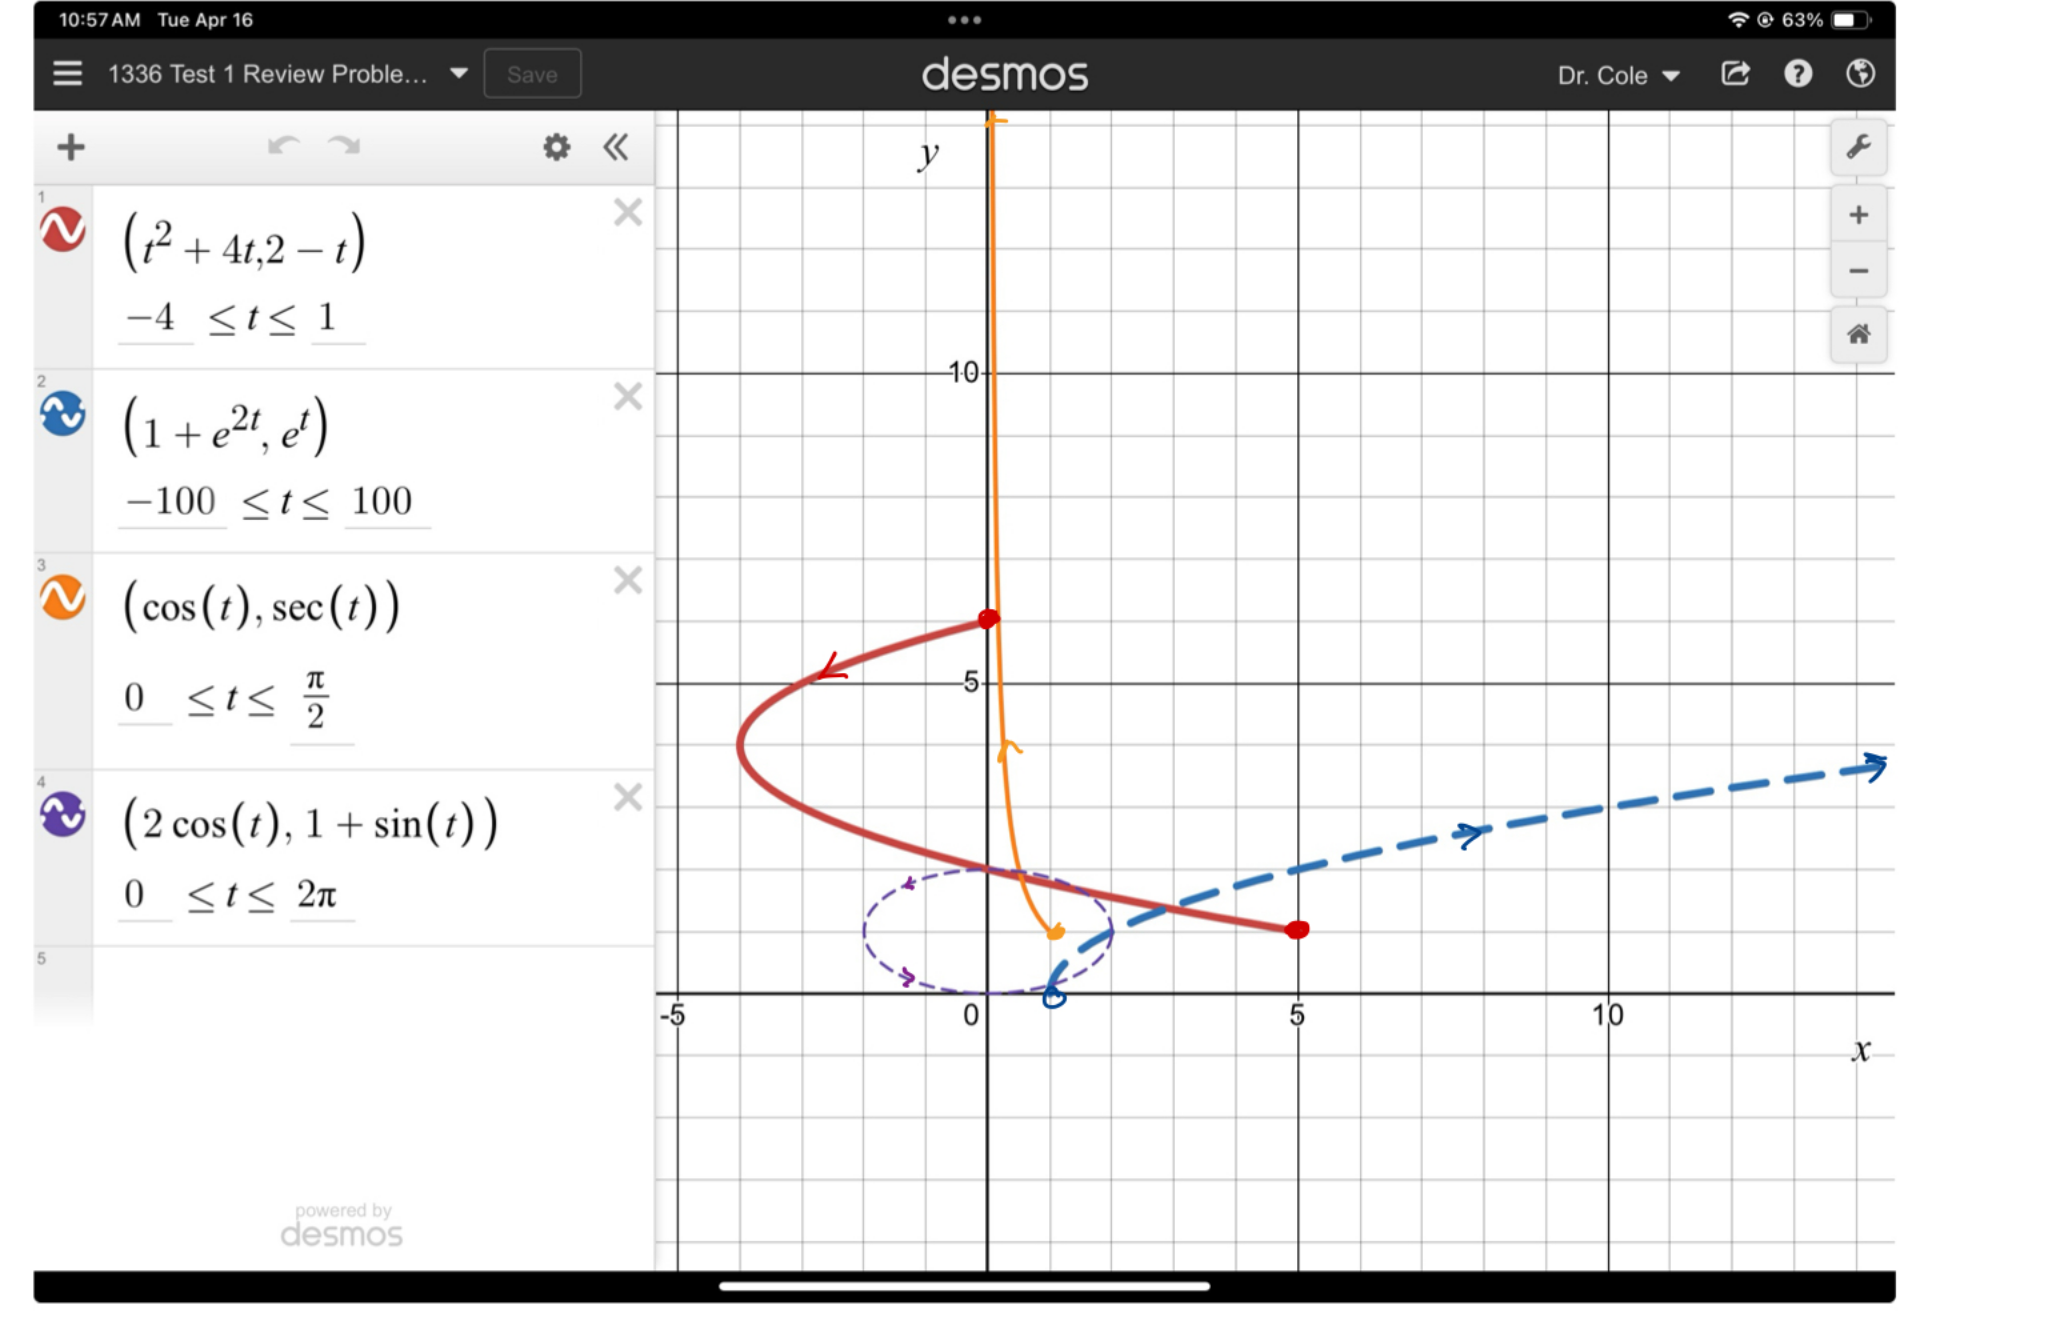
\includegraphics[width=.5\textwidth]{Test1-Rev-Prob1.png}
%\caption{Graphs for Review Problem \ref{prob1}. \url{https://www.desmos.com/calculator/gjt9jxoyci}}\label{fig:prob1}
%\end{figure}
% 
% \ref{prob2a}: \((x,y)=(-2, 2\sqrt{3})\), see Figure \ref{fig:prob2a} for the plotted point, \\
%\ref{prob2b}: \((r, \theta) = (3\sqrt{2}, \tfrac{3\pi}{4}),\ (r, \theta) = (3\sqrt{2}, \tfrac1{11\pi}{4})\ (r, \theta) = (-3\sqrt{2}, \tfrac{7\pi}{4})\);
%
%
%\begin{figure}[!btp]
%\centering
%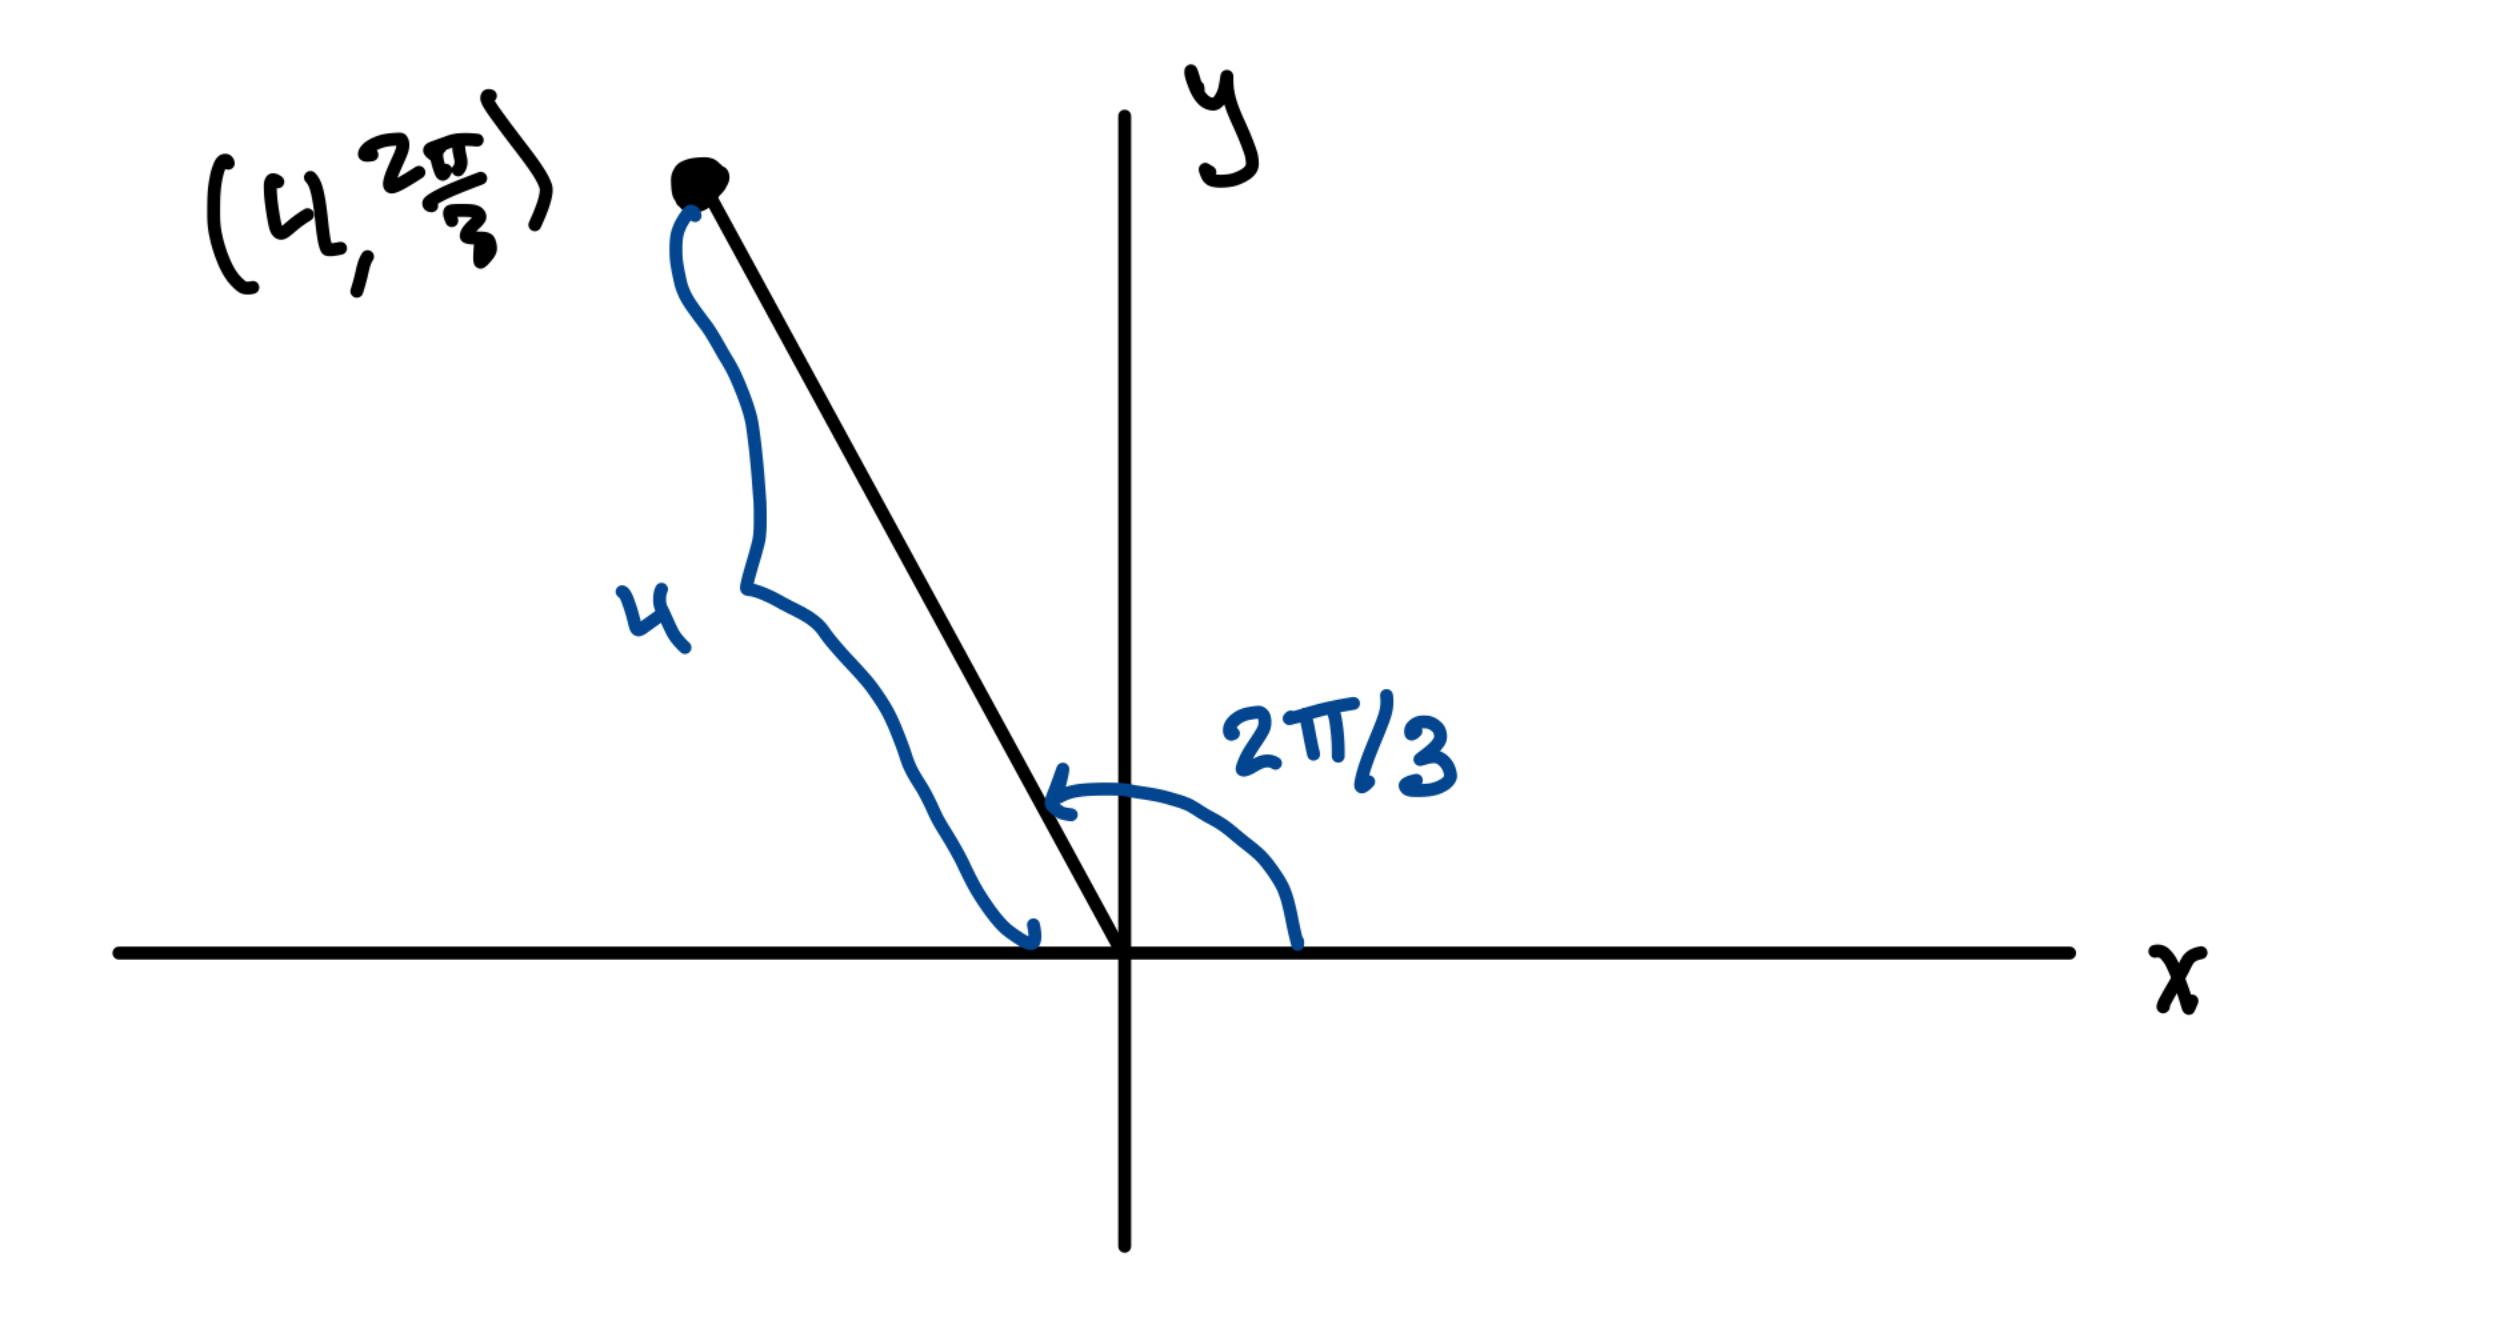
\includegraphics[width=.3\textwidth]{Test1-Rev-Prob2a.png}
%\caption{Plotted point for Review Problem \ref{prob2a}. \url{https://www.desmos.com/calculator/sntaubdedf}}\label{fig:prob2a}
%\end{figure}
% 
%\ref{prob3a}: \(\frac{dy}{dx}=\frac{y'(t)}{x'(t)} = \frac{2t}{1/t} = 2t^2\), when \(t=1\), \(m=2\);  \\
%\ref{prob3b}: \(\frac{dy}{dx}=\frac{y'(t)}{x'(t)} =\frac{2-2t}{3t^2 + 6}\), when \(t=-1\), \(m = \frac{4}{9}\);  \\
% \ref{prob3c}: \(\frac{dy}{dx}=\frac{y'(\theta)}{x'(\theta)} = \frac{\frac{dr}{d\theta}\sin\theta+r\cos\theta}{\frac{dr}{d\theta}\cos\theta - \sin\theta} = \frac{-e^{-\theta}\sin\theta + e^{-\theta}\cos\theta}{-e^{-\theta}\cos\theta - e^{-\theta}\sin\theta} = \frac{\sin\theta - \cos\theta}{\cos\theta+\cos\theta}\), when \(\theta = \pi\), \(m=-1\);  
%
%\ref{prob4a}: \(\frac{dy}{dx} = \frac{y'(t)}{x'(t)} = \frac{1+\sin t}{1+\cos t}\), so \(\frac{d^2y}{dx^2} = \frac{\frac{d}{dt}(\frac{dy}{dx})}{x'(t)} = \frac{\frac{(1+\cos t)\cos t - (1+\sin t)(-\sin t)}{(1+\cos t)^2}}{(1+\cos t)} = \frac{1+\cos t+\sin t}{(1+\cos t)^3}\);  \\
%\ref{prob4b}: \(\frac{dy}{dx} = \frac{y'(t)}{x'(t)} = \frac{1-3t^2}{2t} = \tfrac{1}{2}t^{-1}-\tfrac{3}{2}t\), so \(\frac{d^2y}{dx^2} = \frac{\frac{d}{dt}(\frac{dy}{dx})}{x'(t)} = \frac{ -\tfrac{1}{2}t^{-2}-\tfrac{3}{2}}{2t}\); \\
%
%\ref{prob5a}: \(x'(t) = -2a\sin t + 2a\sin 2t = 2a\sin t(2\cos t - 1) = 0\) when \(t=0, \frac{\pi}{3}, \pi, \frac{5\pi}{3}\),\\
% \(y'(t) = 2a\cos t - 2a\cos 2t = 2a(1+\cos t -2\cos^2 t) = 2a(1-\cos t)(1+2\cos t) = 0\) when \(t=0, \frac{2\pi}{3}, \frac{4\pi}{3}\).\\
%  Horizontal tangent lines at \(t=\frac{2\pi}{3}, \frac{4\pi}{3}\), Vertical tangent lines at \(t=\frac{\pi}{3}, \pi, \frac{5\pi}{3}\), \\
%   L'Hopital's Rule can be used to determine that \(\displaystyle \lim_{t\rightarrow 0}\dfrac{y'(t)}{x'(t)} = 0\), so there is a horizontal tangent there. See Figure \ref{fig:prob5a} for a graph where \(a=1\).\\
%   \textbf{Note:} I would not ask you to do a problem as complicated as this on the test, but a problem with simpler algebra covering the same ideas would be fair game.\\
%   
%\ref{prob5b}: From Figure \ref{fig:prob5a}, we can see that the curve is symmetric, so we can integrate from \(t=\pi\) to \(t=0\) and multiply by 2 to get the entire area:\\ \(A = 2\int_{\pi}^0 (2a\sin t - a \sin 2t) (-2a\sin t + 2a\sin 2t ) dt = 4a^2\int_0^{\pi} (2\sin^2 t + \sin^2 2t - 3\sin t \sin 2t)dt = 6\pi a^2\); 
%
%\begin{figure}[tbp] 
%\centering
%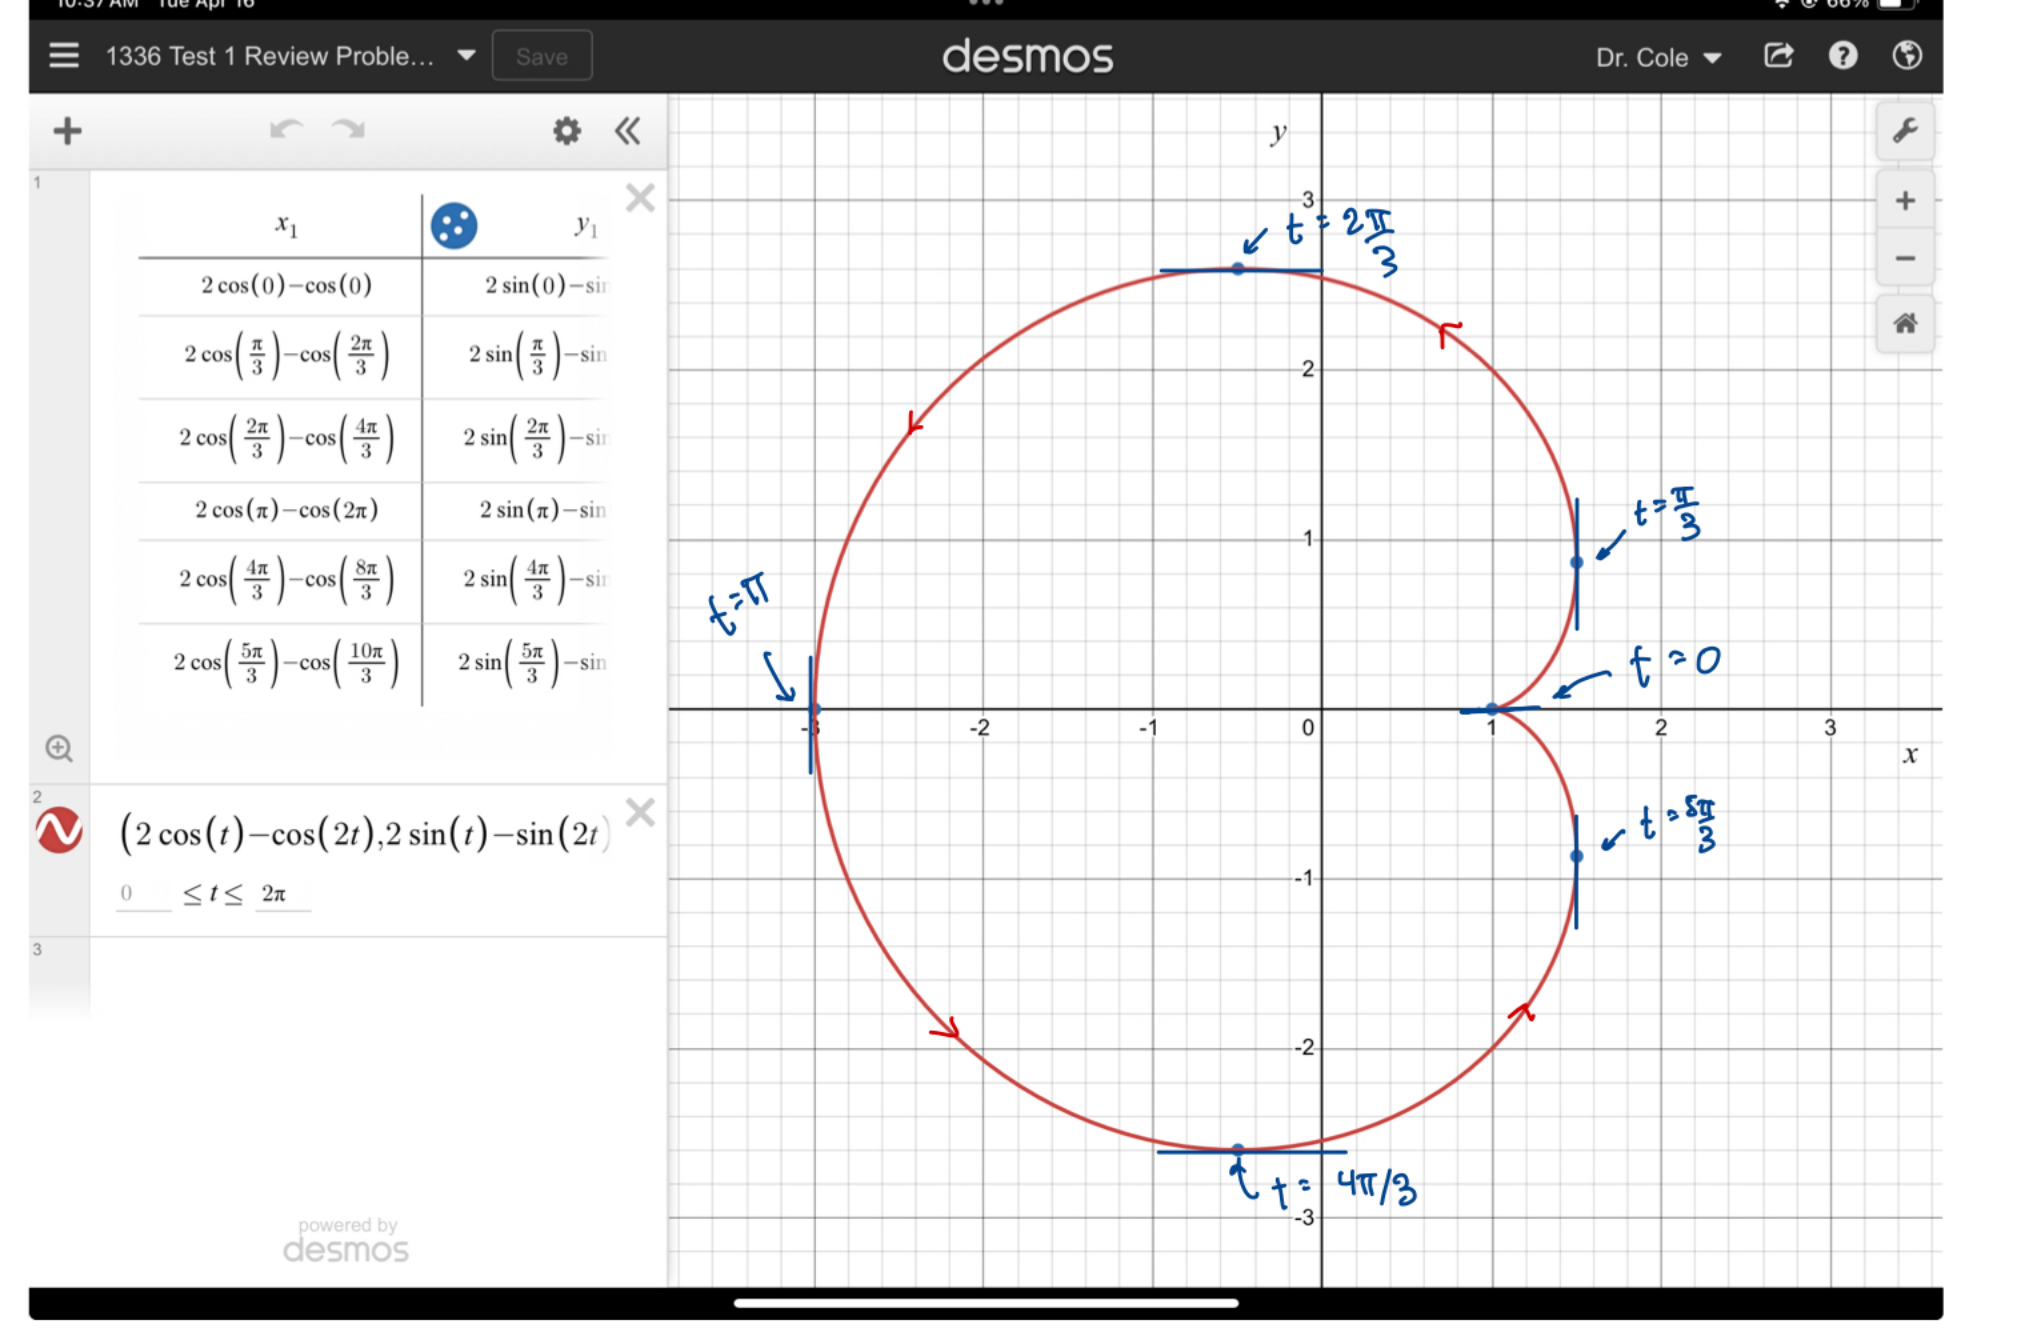
\includegraphics[width=.5\textwidth]{Test1-Rev-Prob5a.png}
%\caption{Graph for Review Problem \ref{prob5a}. \url{https://www.desmos.com/calculator/quki3ltarg}}\label{fig:prob5a}
%\end{figure}
%
%%\ref{prob6}: \textit{This problem was more complicated than I anticipated, so it has been removed from the list!}
%
%\ref{prob7}: The curves intersect when \(2=4\cos \theta\), so \(\cos\theta = \frac{1}{2}\), so \(\theta = \pm \frac{\pi}{3}\). The points of intersection are \((r,\theta) = (2, \pm\frac{\pi}{3})\). See Figure \ref{fig:prob7} for reference; 
%
%
%\begin{figure}[tbp] 
%\centering
%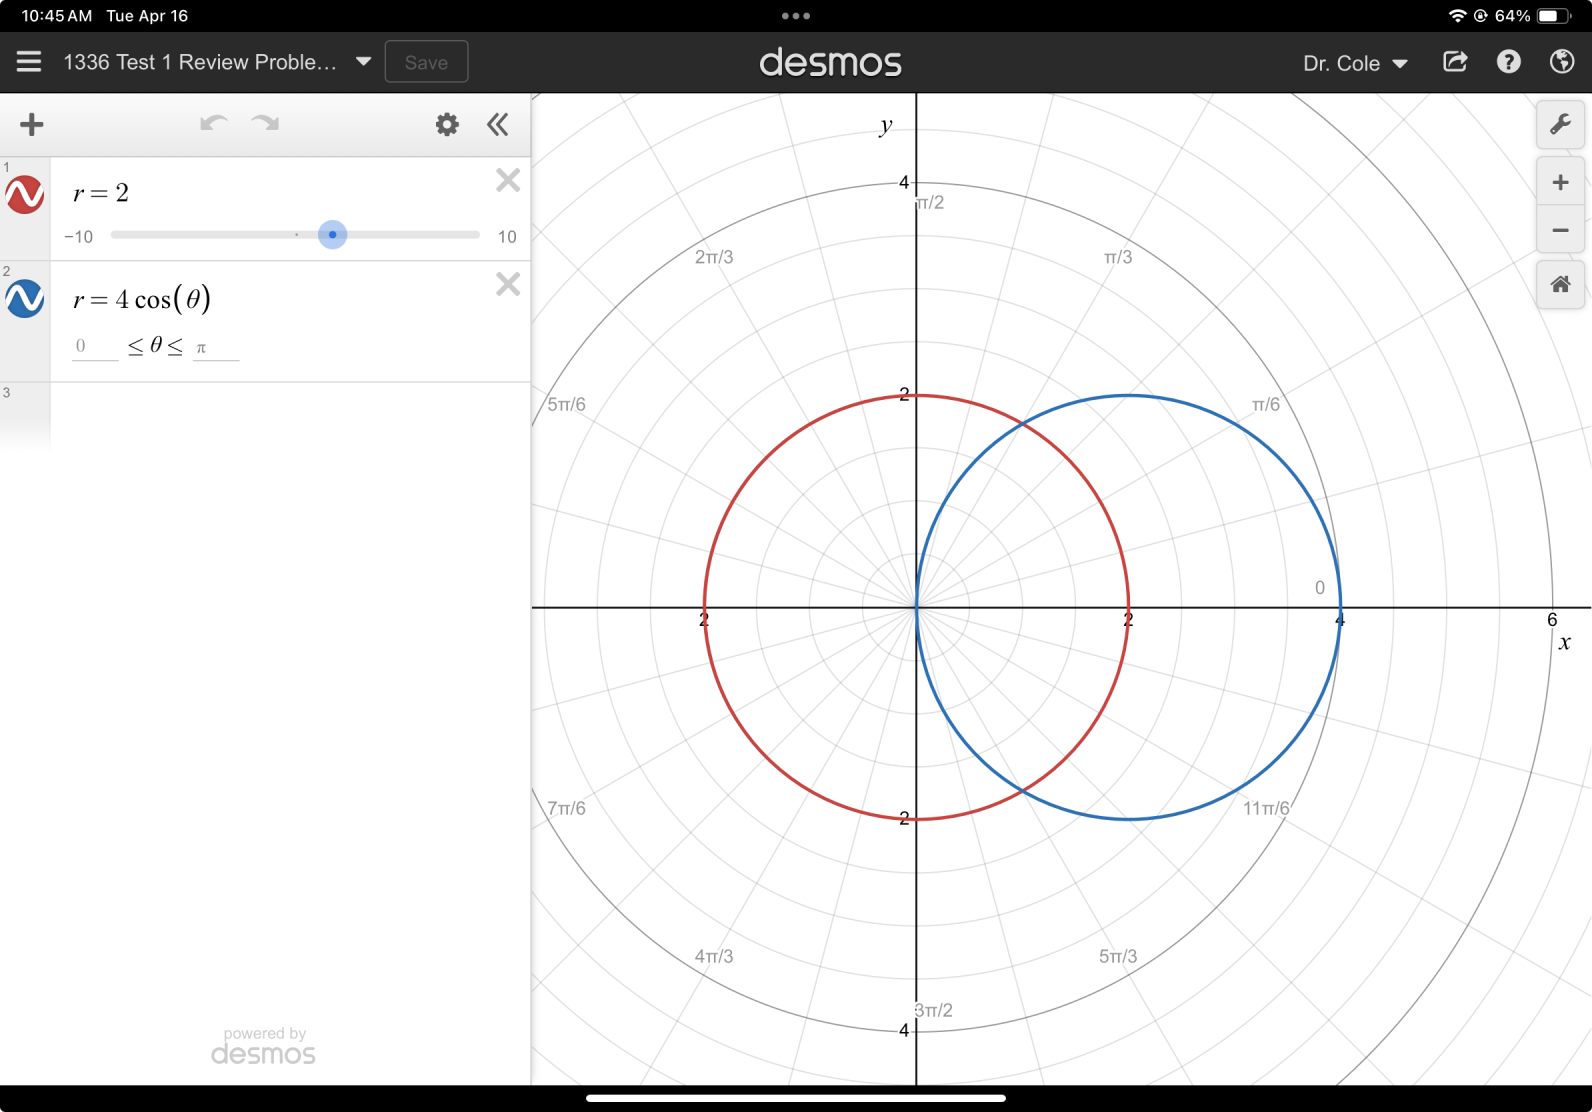
\includegraphics[width=.5\textwidth]{Test1-Rev-Prob7.png}
%\caption{Graph for Review Problem \ref{prob7}. \url{https://www.desmos.com/calculator/65wgr46r3i}}\label{fig:prob7}
%\end{figure}
%
%\ref{prob8a}: \(L = \int_0^2 \sqrt{(\frac{dx}{dt})^2+(\frac{dy}{dt})^2} dt = \int_0^2 \sqrt{36t^2+36t^4} dt = \int_0^2 6t\sqrt{1+t^2}\ dt = 2(5\sqrt{5}-1) \),\\
% \textit{Hint:} try a rationalizing substitution;
% 
%\ref{prob8b}: \(L = \int_{\pi}^{2\pi} \sqrt{(r)^2+(\frac{dr}{d\theta})^2} d\theta = \int_{\pi}^{2\pi} \sqrt{\frac{1}{\theta^2}+\frac{1}{\theta^4}} d\theta = \int_{\pi}^{2\pi} \frac{\sqrt{\theta^2+1}}{\theta^2} d\theta  \), \textit{(set-up only)}; 
%
%%\ref{prob9}: The radius is the distance from the center to the point: \\
%%\(R = \sqrt{(6+1)^2+(-2-2)^2+(4-1)^2} = \sqrt{74}\), then the formula for the sphere is:\\
%% \((x+1)^2+(y-2)^2+(z-1)^2 = 74\); 
%
%\ref{prob10a}: \(\u\cdot\v = ||\u||\ ||\v||\ \cos \tfrac{\pi}{4} = 3\sqrt{2}\),
%\ref{prob10b}: \(||\u\times \v|| = ||\u||\ ||\v||\ \sin \tfrac{\pi}{4} = 3\sqrt{2}\), \\
%\ref{prob10c}: \(\u \times \v\) points out of the page; 
% 
% \pagebreak
% 
% \ref{prob11a}: \(2\a + 3\b = \<11, -4, -1\>\), 
%  \ref{prob11b}: \(||\b|| = \sqrt{9+4+1} = \sqrt{14}\) , 
%  \ref{prob11c}: \(\a \cdot \b = -1\), \\
%  \ref{prob11i}:  \(\text{comp}_{\a} \b = \frac{\a\cdot\b}{||\a||} =\frac{-1}{\sqrt{6}} \), 
%  \ref{prob11j}: \(\text{proj}_{\a} \b = \frac{\a\cdot\b}{||\a||^2}\a =\frac{-1}{6}\<1, 1, -2\>\),  \\
%  \ref{prob11k}: \(\theta = \cos^{-1}(\frac{\a\cdot\b}{||\a||\ ||\b||}) = \cos^{-1}(\frac{-1}{\sqrt{6}\sqrt{14}})\approx 1.68\ \text{radians}\) ;  
%
% \ref{prob12}: Solve for \(x\):  \(\<3, 2, x\> \cdot \<2x, 4, x\> =6x+8+x^2 =(x+4)(x+2)= 0 \), so \(x=-4,\ x=-2\); 
% 
% \ref{prob13}: \(\vec{D} = \<5-1,3-0,8-2\>=\<4, 3, 6\>\), so\\
%  \(W = \vec{F}\cdot \vec{D} = \<3, 5, 10\>\cdot\<4, 3, 6\> = 12+15+60 = 87\ N\ m = 87\ J\);
%  
%  \ref{prob14}: See Figure \ref{fig:prob14} for graphs, 
%  \ref{prob14a}: vertical plane where \(x=3\), 
%\ref{prob14b}: plane perpendicular to \(xz\)-plane where \(x=z\), 
% \ref{prob14c}: parabolic cylinder with vertex along the \(x\)-axis, opening to the right; 
% 
% 
% \begin{figure}[btp]
% \centering
% 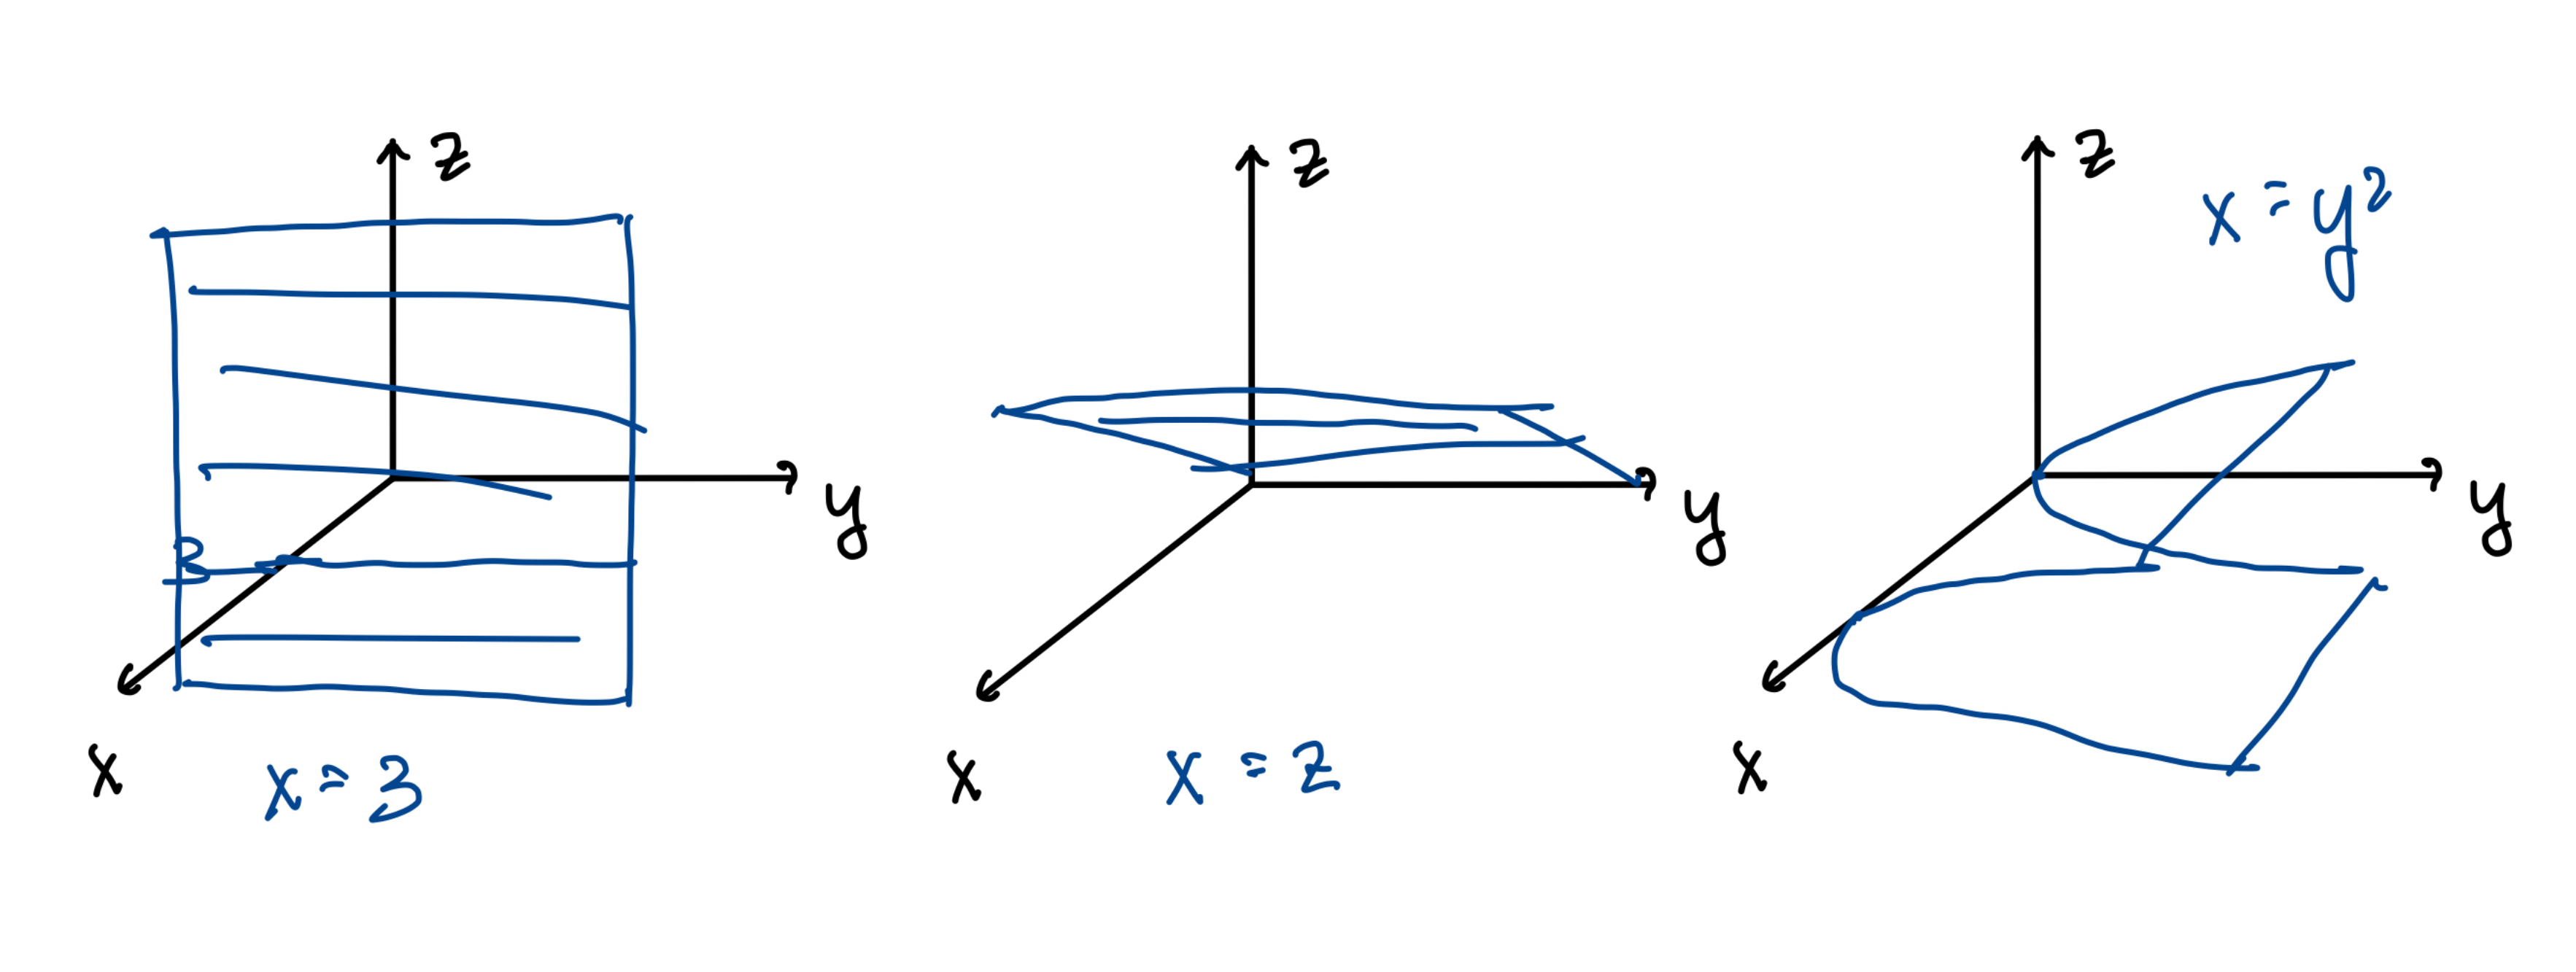
\includegraphics[width=\textwidth]{Test1-Rev-Prob14.png}
% \caption{Graphs for Review Problem \ref{prob14}}\label{fig:prob14} 
% \end{figure}
%
\label{lastpage}

\end{document}